\chapter{Localization and Reversal of Paratropic Ring Currents in Molecules with Formal Anti-Aromatic Electron Counts}
\label{chap_indacene}
\footnotetext{Reproduced with permission: ``Localization and Reversal of Paratropic Ring Currents in Molecules with Formal Anti-Aromatic Electron Counts'', \mbox{R. W. A. Havenith}, \mbox{J. J. Engelberts}, \mbox{P. W. Fowler}, \mbox{E. Steiner}, \mbox{J. H. van Lenthe} and \mbox{P. Lazzeretti}, \textit{Phys. Chem. Chem. Phys.} \textbf{2004}, \textit{6}, 289-294.\ \ \ \copyright 2004 PCCP Owner Societies.}

\ifthenelse{\boolean{wholethesis}}{\relax}{\begin{center}\textit{Generated on \today\ at \currenttime}\end{center}}

\noindent\textbf{Abstract:} The aromatic character of the six smallest members of the $\alpha$,$\omega$-bicyclopenta-diene-polyacene series (\textbf{1}($n$)) has been assessed using magnetic and energetic criteria. Current density maps (CTOCD-\textit{DZ}/6-31G**//B3LYP/6-31G**) show that, along the series, the ring current changes from paratropic in pentalene (\textbf{1}(\textit{0})) and $s$-indacene (\textbf{1}(\textit{1})), through quenched in \textbf{1}(\textit{2}) and \textbf{1}(\textit{3}), to diatropic in \textbf{1}(\textit{4}) and \textbf{1}(\textit{5}). These changes are rationalized in terms of orbital contributions to current. Valence Bond calculations (VB/\mbox{6-31G}// B3LYP/\mbox{6-31G**}) in which the $\pi$ system is composed of strictly atomic $p$ orbitals, show that the electronic structures in these homologous series can be described in terms of the two closed-shell Kekul\'e resonance structures for the smallest molecules, but that in the larger molecules allyl-polyacene-allyl bi-radical structures prevail, owing to the larger resonance energies. This trend in electronic structure parallels the switch from paratropic to diatropic character.

\newpage

\section{Introduction}

\lettrine{\initial{I}}{}n organic chemistry, the term aromaticity is frequently used to classify a compound according to its structure and/or properties. Different criteria for aromaticity exist: electron-counting (4$n$+2 \textit{vs.} 4$n$ $\pi$ electrons), geometric (bond length equalization), energetic (extra stabilization with respect to a hypothetical, localized, reference molecule), and magnetic (ability to sustain a diatropic ring current)  \cite{r01,r02,r03,r04}. It should be noted that the H\"uckel 4$n$+2 rule is derived for monocycles only, and is not directly applicable to other systems. If, however, the closed-shell Lewis structures for a particular molecule are identical with those of a 4$n$+2/4$n$ carbon monocycle, the aromatic character of that molecule is expected to be similar to that of the parent monocycle. A study of the induced current density for bicyclic molecules illustrated this similarity for aromaticity on the magnetic criterion  \cite{r05}.

Molecules for which the different criteria of aromaticity lead to different conclusions offer interesting targets for further investigation. A typical example is $s$-indacene \textbf{1}(\textit{1}), Chart 1, $n$ = 1).
\begin{figure}[htdp]
\center
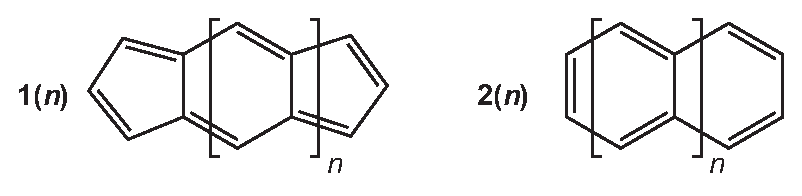
\includegraphics[width=3in]{indacene/figures/chart1.eps}\\
\textbf{Chart 1}
\end{figure}
$s$-Indacene itself is a very reactive molecule  \cite{r06} ('anti-aromatic'), and an \mbox{X-ray} crystal structure is available only for its tetra-\textit{tert}-butyl derivative  \cite{r07} from which $D_\mathrm{2h}$ symmetry was deduced ('aromatic'). The molecule has been the subject of several theoretical studies, \textit{e.g.} on $\pi$ distortivity and double-bond localization  \cite{r08}, geometry  \cite{r09,r10}, electronic spectrum  \cite{r11,r12}, and aromaticity  \cite{r13,r14}. $s$-Indacene has 12 $\pi$ electrons (an 'anti-aromatic' count), it possesses $D_\mathrm{2h}$ symmetry in its equilibrium geometry ('aromatic' bond equalization)  \cite{r10}, the aromatic stabilization energy (ASE) is 45.1 kJ/mol (a 'non-aromatic' value), and the nucleus-independent chemical shift (NICS)  \cite{r15} values for the five-membered rings are +25.8 ppm and +20.8 ppm for the central benzene-ring (both 'anti-aromatic' values)  \cite{r13}. A detailed study of the current density, induced by an external magnetic field shows that $s$-indacene sustains a paratropic ring current, which indicates anti-aromaticity  \cite{r14}.

Pentalene is different from $s$-indacene; the bridging benzene ring is absent and distortion to $C_\mathrm{2h}$ symmetry is predicted  \cite{r16,r17}. The question of how the induced current density, and thus the aromatic character, for the $\alpha$,$\omega$-bicyclopentadiene-polyacene series, change on elongation of the bridging benzeno-moiety, will be explored here.

For the closely related polyacene-series (\textbf{2}($n$), Chart 1), the magnetic properties and in particular the induced current density have been studied in detail  \cite{r18,r19}. For this series, a strong, diatropic, perimeter current is observed, which is concentrated in the central benzene rings  \cite{r18}. A similar behavior might be expected for series \textbf{1}($n$), implying that a molecule with an anti-aromatic electron count could behave like one with 4$n$+2 \mbox{$\pi$ electrons}. If so, the $\pi$ system of \textbf{1} should split into an aromatic system with 4$n$+2 \mbox{$\pi$ electrons} and two systems of 2$m$+1 $\pi$ electrons (Chart 2).
\begin{figure}[htdp]
\center
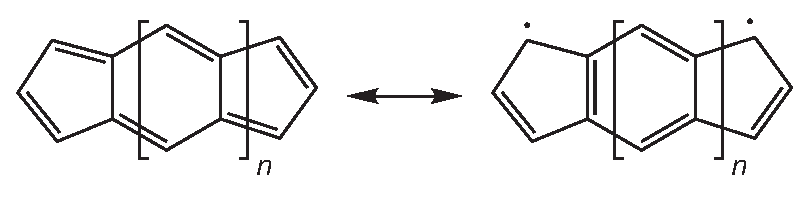
\includegraphics[width=3in]{indacene/figures/chart2.eps}\\
\textbf{Chart 2}
\end{figure}
This transition is expected to occur when the loss of energy due to the formation of a bi-radical system is balanced by the stabilization gain from resonance in the aromatic $\pi$ system.

In this chapter it will be shown how the balance between the two possible Kekul\'e-like and the bi-radical Valence Bond structures changes upon elongation of the chain, and the
concomitant changes in the current density induced by a magnetic field are explored. For larger systems, the bi-radical structures become more important, and the paratropic ring current reverses.

\section{Methods}

Geometries of \textbf{1}($n$), with $n$ = 0--5, were optimized at the B3LYP/6-31G** level of theory with imposed $D_\mathrm{2h}$ and $C_\mathrm{2h}$ symmetry, using GAMESS-UK  \cite{r20}. At the B3LYP/6-31G** level, the $D_\mathrm{2h}$ structures for \textbf{1}(\textit{0}) and \textbf{1}(\textit{1}) correspond to the transition states that connect the two symmetry-equivalent localized $C_\mathrm{2h}$ minima. The geometries used in all following calculations were the B3LYP/6-31G** $D_\mathrm{2h}$ optima. The magnetic properties of the molecules \textbf{1}($n$) were computed with the ipsocentric CTOCD-\textit{DZ} (continuous transformation of current density-\textit{diamagnetic zero}) method  \cite{r21,r22,r23,r24}, at the coupled Hartree--Fock level of theory, with the SYSMO program  \cite{r25} in the 6-31G** basis set. The current density induced by a magnetic field directed perpendicular to the molecular plane is plotted in a plane 1 $a_0$ above and parallel to the molecular plane (where the $\pi$ current density is close to its maximum  \cite{r18}); arrows represent in-plane projections of the current density and diatropic circulation is shown anti-clockwise.

Model H\"uckel--London ring currents  \cite{r26,r27} were also calculated. Bond-bond polarizabilities for estimation of $\pi$ electron distortivity were calculated by literature procedures   \cite{r08,r17,r28,r29,r30}. Valence Bond (VB) calculations were performed using the TURTLE program   \cite{r31}, as integrated in the GAMESS-UK program  \cite{r20}, in the 6-31G basis set. The $\pi$ system is described by strictly atomic, singly occupied, $p$ orbitals, optimized for a free carbon atom; $\sigma$ orbitals are kept frozen and were taken from a preceding RHF calculation. The resonance energy is defined, according to Pauling  \cite{r32,r33}, as the difference between the total VB energy and the energy of the most stable structure in the same calculation.

\section{Results and Discussion}

\subsection{Geometries and $\pi$ Distortivity}

The total energies obtained for the $D_\mathrm{2h}$ and $C_\mathrm{2h}$ symmetric structures are presented in Table \ref{ch7.tab01}, together with their energy differences.
\begin{table}[ht]
\caption{B3LYP/6-31G** total energies (in $E_\mathrm{h}$) for compounds \textbf{1}($n$) in $D_\mathrm{2h}$ and $C_\mathrm{2h}$ symmetry, and energy difference $\Delta E = E(\mathrm{D}_{2h})-  E(\mathrm{C}_{2h})$ (kJ/mol)}
\begin{center}
\begin{tabular}{l r r r }
\hline
Molecule &
$E$ / $E_\mathrm{h}$ ($D_\mathrm{2h}$)&
$E$ / $E_\mathrm{h}$ ($C_\mathrm{2h}$)&
$\Delta E$ / (kJ/mol)\\
\hline
\textbf{1}(\textit{0}) & -308.3675289 & -308.3790512 & 30.22\\
\textbf{1}(\textit{1}) & -462.0405516 & -462.0407734 & 0.59\\
\textbf{1}(\textit{2}) & -615.6869635 & ${}^\mathrm{a}$ &\\
\textbf{1}(\textit{3}) & -769.3271108 & ${}^\mathrm{a}$ &\\
\textbf{1}(\textit{4}) & -922.9638116 & ${}^\mathrm{a}$ &\\
\textbf{1}(\textit{5}) & -1076.5989777 & ${}^\mathrm{a}$ &\\
\hline
\end{tabular}
\\
\flushleft
${}^\mathrm{a}$ No $C_\mathrm{2h}$ minimum, geometry optimization starting from $C_\mathrm{2h}$ leads to a $D_\mathrm{2h}$ symmetric geometry.
\end{center}
\label{ch7.tab01}
\end{table}
The geometries of the two smallest members (\textbf{1}(\textit{0}) and \textbf{1}(\textit{1})) of this series distort from the ideal $D_\mathrm{2h}$ to $C_\mathrm{2h}$ symmetry. For pentalene, this is in accordance with the available experimental data (see for example ref.   \cite{r34}). However, 1,3,5,7-tetra-\textit{tert}-butyl-$s$-indacene possesses $D_\mathrm{2h}$ symmetry in the solid state  \cite{r07}. The difference in energy between the $D_\mathrm{2h}$ and $C_\mathrm{2h}$ structures for \textbf{1}(\textit{1}) is only 0.59 kJ/mol, indicating a very shallow minimum, in agreement with previous theoretical treatments  \cite{r10,r13,r14}. At the CASPT2 level of theory, a minimum with $D_\mathrm{2h}$ symmetry can be located  \cite{r01}.

The higher homologues in this series possess $D_\mathrm{2h}$ symmetry, and no $C_\mathrm{2h}$ minima were located at this level. From the geometric criterion for aromaticity alone, a change in aromatic character is evident, with a change from anti-aromatic to aromatic along the series.

The distortive propensity of the $\pi$ electrons of simple conjugated hydrocarbons can already be predicted at the level of H\"uckel theory: the eigenvectors of the $\pi$ bond-bond polarizability matrix indicate the directions of distortivity of the $\pi$ electrons  \cite{r08,r17,r29,r30}. Empirically, it is found that when the magnitude of the maximum eigenvalue ($|\beta\lambda^{\pi}_{max}|$) of this matrix is larger than the critical value of 1.8$|\beta|^{-1}$, the molecule will distort  \cite{r17,r29}. In Table \ref{ch7.tab02}, the maximum eigenvalues of the $\pi$ bond-bond polarizability matrix are presented.
\begin{table}[ht]
\caption{Magnitude of the maximum eigenvalue ($|\beta\lambda^{\pi}_{max}|$) of the $\pi$ bond-bond polarizability matrix for species \textbf{1}(\textit{n})}
\begin{center}
\begin{tabular}{l l l l }
\hline
Molecule &
$|\beta\lambda^{\pi}_{max}|$&
Molecule &
$|\beta\lambda^{\pi}_{max}|$\\
\hline
\textbf{1}(\textit{0}) & 2.357 & \textbf{1}(\textit{3}) & 1.311\\
\textbf{1}(\textit{1}) & 1.573 & \textbf{1}(\textit{4}) & 1.278\\
\textbf{1}(\textit{2}) & 1.381 & \textbf{1}(\textit{5}) & 1.260\\
\hline
\end{tabular}
\\
\flushleft
${}^\mathrm{a}$ No $C_\mathrm{2h}$ minimum, geometry optimization starting from $C_\mathrm{2h}$ leads to
a $D_\mathrm{2h}$ symmetric geometry.
\end{center}
\label{ch7.tab02}
\end{table}
Only for pentalene (\textbf{1}(\textit{0})) is the maximum eigenvalue magnitude of 2.357$|\beta|^{-1}$ larger than the critical threshold, and indeed pentalene distorts from $D_\mathrm{2h}$ to $C_\mathrm{2h}$ symmetry  \cite{r16}. A gradual decrease in the magnitude of $|\beta\lambda^{\pi}_{max}|$ is seen with increasing length of the molecule. $s$-Indacene has $|\beta\lambda^{\pi}_{max}|$ close to the critical value (1.573)  \cite{r08}, and at B3LYP/6-31G** (and RHF  \cite{r09}), the $C_\mathrm{2h}$ structure prevails. Values for the other compounds of the series \textbf{1}(\textit{n}) with {$n >$ 2} are well below the critical threshold, and at the B3LYP/6-31G** level of theory, these molecules do indeed have $D_\mathrm{2h}$ symmetry.

\subsection{Current Density Maps}

The CTOCD-DZ $\pi$ current density maps for \textbf{1}(\textit{n}) in $D_\mathrm{2h}$ symmetry are shown in Fig. \ref{ch7.fig01}
\begin{figure}[htp]
\center
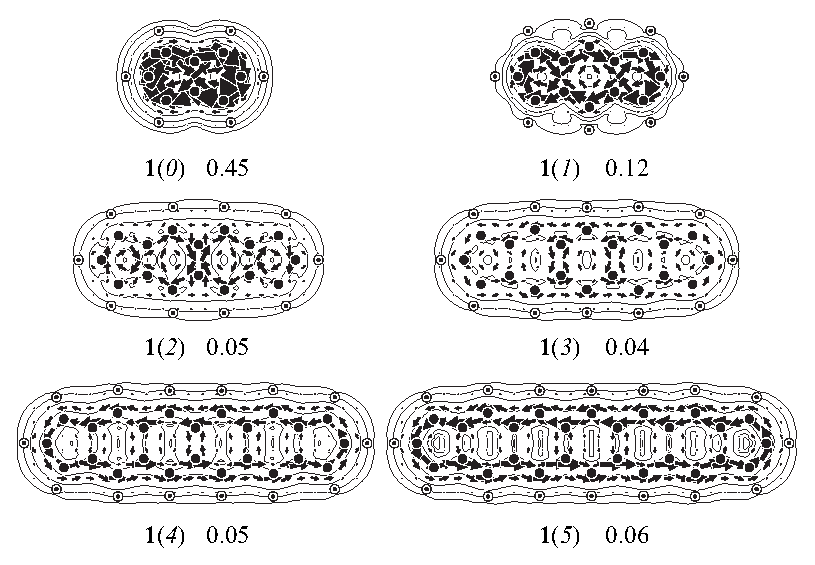
\includegraphics{indacene/figures/figure1.eps}
\caption{$\pi$ current density maps for the series \textbf{1}(\textit{n}), plotted 1 $a_0$ above the molecular plane. The maximum of the current density ($j_{max}$/au) is indicated below each map. Anti-clockwise circulation is diatropic/clockwise paratropic.}
\label{ch7.fig01}
\end{figure}
 together with a note of the maximum value of the $\pi$ current density in the plotting plane ($j_{max}$). Total ($\sigma$+$\pi$) maps are shown in Fig. \ref{ch7.fig02}. For pentalene (\textbf{1}(\textit{0})) and $s$-indacene (\textbf{1}(\textit{1})), a strong, paratropic, perimeter current is visible  \cite{r05,r14}.
\begin{figure}[hbp]
\center
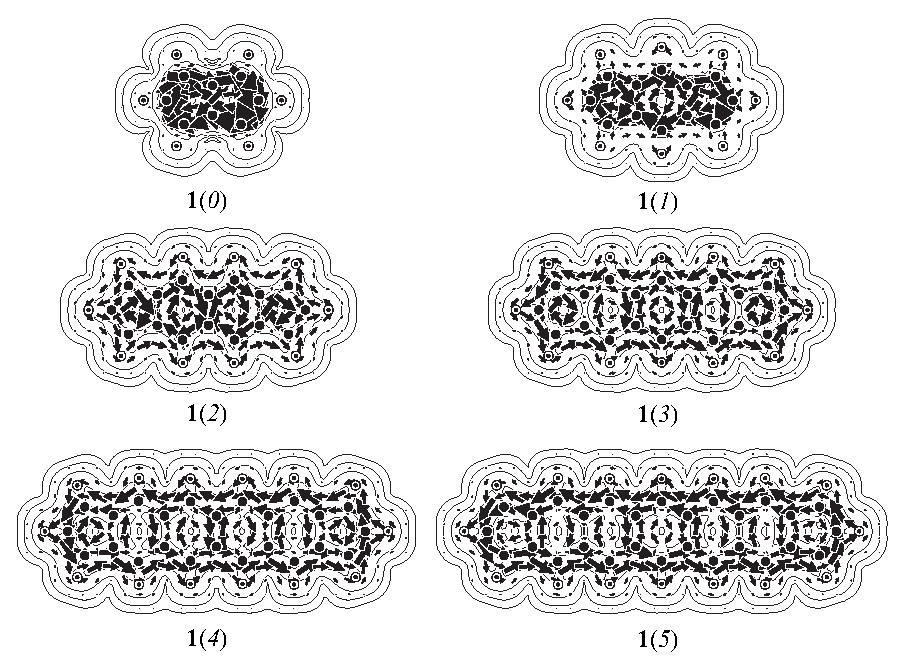
\includegraphics[scale=0.8]{indacene/figures/figure2.eps}
\caption{Total ($\sigma$ + $\pi$) current density maps for the series \textbf{1}(\textit{n}), plotted 1 $a_0$ above the molecular plane. Plotting conventions as Fig. \ref{ch7.fig01}.}
\label{ch7.fig02}
\end{figure}
The current density for \textbf{1}(\textit{2}) remains similar to those of \textbf{1}(\textit{0}) and \textbf{1}(\textit{1}), though weaker. In contrast, for \textbf{1}(\textit{3}) the paratropic current is quenched and replaced by localized diatropic bond currents, and a weak diatropic perimeter circulation grows in. The intensity of the current is reflected in the value of $j_{max}$. For the larger homologues, the diatropic current strengthens. When the paratropic $\pi$ current density starts to break down (\textbf{1}(\textit{2}) and \textbf{1}(\textit{3})), a sharp drop in $j_{max}$ is seen, as is a (smaller) increase when the current reverses to give a diatropic $\pi$ ring current.

The total current density maps shown in Fig. \ref{ch7.fig02}, are broadly similar to the $\pi$ maps, with the usual additional characteristics of $\sigma$ current: diatropic flow on the outside of the molecule, and paratropic flow around the centre of each ring, as a consequence of superposed local diatropic circulations around $\sigma$ bonds \cite{r18}. Insight into the changes of the ring current patterns upon chain elongation is provided by a breakdown of the total induced current density in orbital contributions  \cite{r35,r36}.
\clearpage
\newpage
The orbital-by-orbital analysis shown in Figures \ref{ch7.fig03a}, \ref{ch7.fig03b} and \ref{ch7.fig03c}  show a clear change in the individual roles of the frontier molecular orbitals.
\begin{figure}[htp]
\center
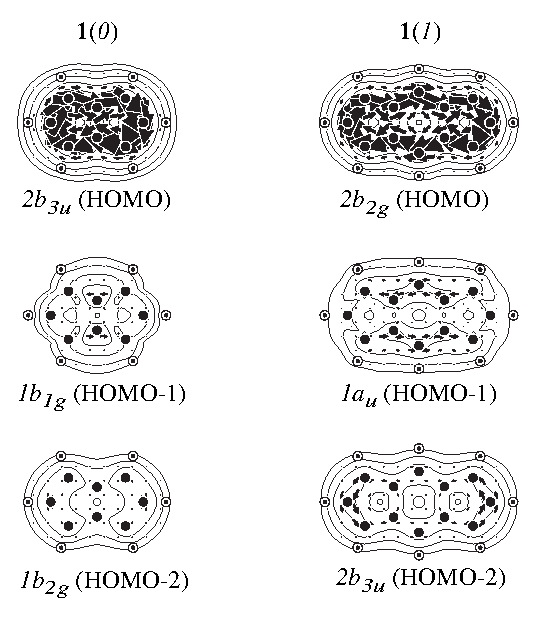
\includegraphics{indacene/figures/figure3a.eps}
\caption{Decomposition of the $\pi$ current density into orbital contributions for \textbf{1}(\textit{0}) and \textbf{1}(\textit{1}). Only the orbitals with significant contributions to the $\pi$ current density are shown. Plotting conventions as Fig. \ref{ch7.fig01}.}
\label{ch7.fig03a}
\end{figure}
The paratropic currents for \textbf{1}(\textit{0}) and \textbf{1}(\textit{1}) (Fig. \ref{ch7.fig03a}) are dominated by HOMO ($2b_\mathrm{3u}$ and $2b_\mathrm{2g}$) contributions. In accordance with previous calculations  \cite{r14,r35,r36} the induced current density in these compounds is dominated by the HOMO contribution, and diatropic contributions from the lower lying $1b_\mathrm{1g}$ and $1b_\mathrm{2g}$ for \textbf{1}(\textit{0}) and $1a_\mathrm{u}$ and $2b_\mathrm{3u}$ for \textbf{1}(\textit{1}) are very weak.

For the larger homologues \textbf{1}(\textit{n}) (Figures \ref{ch7.fig03b} and \ref{ch7.fig03c}), the paratropic contribution of the highest occupied $b_\mathrm{3u}$ orbital ($b_\mathrm{2g}$ for odd $n$) decreases rapidly in strength, and an accompanying increase is found in the diatropic contributions of the occupied $b_\mathrm{1g}$ and $b_\mathrm{2g}$ molecular orbitals ($a_\mathrm{u}$ and $b_\mathrm{3u}$ for odd $n$) near the frontier.
\begin{figure}[htp]
\center
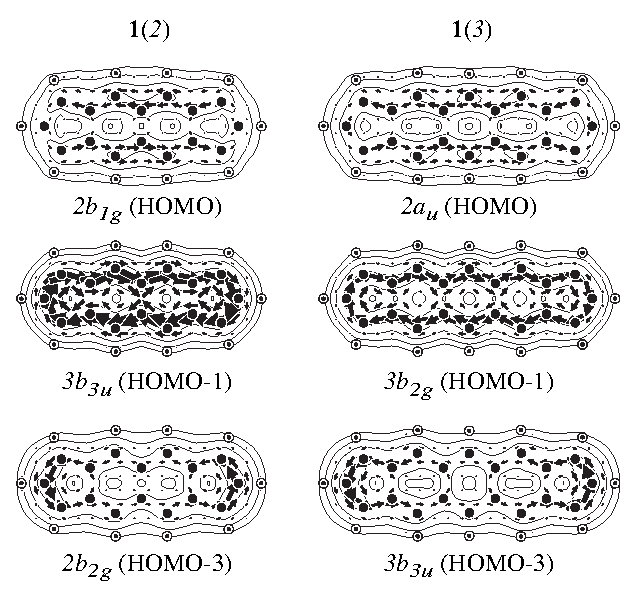
\includegraphics{indacene/figures/figure3b.eps}
\caption{Decomposition of the $\pi$ current density into orbital contributions for \textbf{1}(\textit{2}) and \textbf{1}(\textit{3}). Only the orbitals with significant contributions to the $\pi$ current density are shown. Plotting conventions as Fig. \ref{ch7.fig01}.}
\label{ch7.fig03b}
\end{figure}
\begin{figure}[hbp]
\center
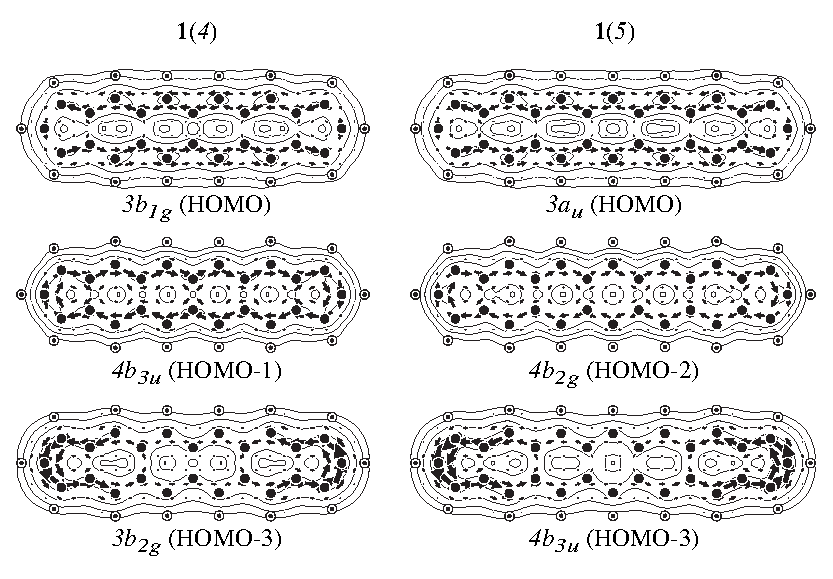
\includegraphics{indacene/figures/figure3c.eps}
\caption{Decomposition of the $\pi$ current density into orbital contributions for \textbf{1}(\textit{4}) and \textbf{1}(\textit{5}). Only the orbitals with significant contributions to the $\pi$ current density are shown. Plotting conventions as Fig. \ref{ch7.fig01}.}
\label{ch7.fig03c}
\end{figure}
Superposition of the orbital contributions results in the observed reversal of the characteristic anti-aromatic paratropic $\pi$ current. A rationale for these changes follows from consideration of the changes in the frontier molecular orbitals. These changes are already evident at the level of H\"uckel molecular orbital theory, as H\"uckel-London theory  \cite{r26,r27} is capable of reproducing the observed patterns of \textit{ab initio} current density in these cases, as is now shown.
\clearpage
\newpage
The H\"uckel-London  \cite{r26,r27} maps of induced current density for the series \textbf{1}(\textit{n}) are shown in Fig. \ref{ch7.fig04}.
\begin{figure}[hb]
\center
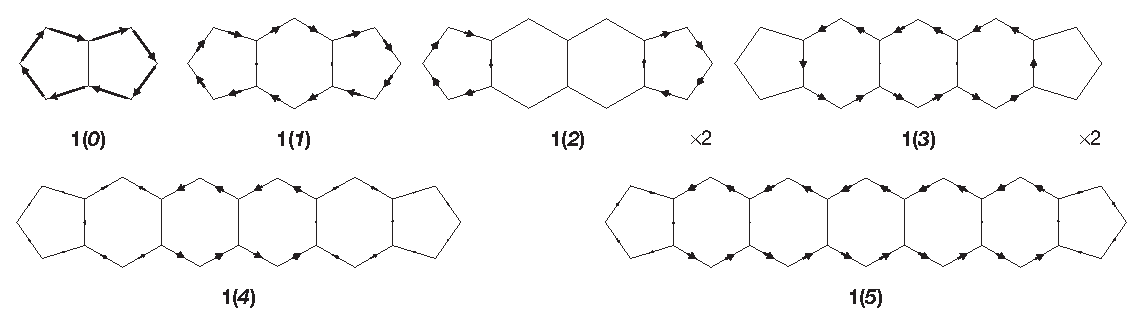
\includegraphics[scale=0.78]{indacene/figures/figure4.eps}
\caption{Schematic ring current patterns obtained for the series \textbf{1}(\textit{n}) using the H\"uckel-London approach \cite{r26,r27}. The arrows for \textbf{1}(\textit{2}) and \textbf{1}(\textit{3}) are scaled by a factor of two compared to the other molecules in the series.}
\label{ch7.fig04}
\end{figure}
For pentalene, as expected, a strong, paratropic current is predicted. The strength of the current decreases with increasing $n$, and for {$n =$ 2}, the paratropic current has vanished, in accordance with the \textit{ab initio} maps, which indicate that localization has set in by this value of $n$. By {$n =$ 3}, a weak diatropic current starts to flow, avoiding the pentagons. For larger $n$ this diatropic current increases in strength, and concentrates on the polyacene moiety.

A rationalization of the changes in the ring current patterns can be given by envisaging the molecule as being derived from a parent monocycle by cross-linking, and considering the concomitant changes in the frontier molecular orbitals. For example, pentalene (\textbf{1}(\textit{0})) can be regarded as derived from a parent $D_\mathrm{8h}$ planar cyclooctatetraene in which a cross-link is made between atoms 1 and 5. This link splits the degenerate $e_\mathrm{2u}$ pair into a bonding $b_\mathrm{3u}$ orbital and a non-bonding $a_\mathrm{u}$ LUMO according to the coefficients on centers 1 and 5. The origin of the paratropic ring current of pentalene therefore lies in the rotationally allowed HOMO ($b_\mathrm{3u}$) $\rightarrow$LUMO ($a_\mathrm{u}$) transition   \cite{r05,r35,r36} of perturbed cyclooctatetraene. If the series \textbf{1}(\textit{n}) is regarded as derived from the parent monocycle by periodic cross-linking, the HOMO and LUMO arise from splitting of the half-filled degenerate pair of the monocycle into a $b_\mathrm{3u}$ occupied and an $a_\mathrm{u}$ unoccupied orbital (even $n$) or a $b_\mathrm{2g}$ occupied and a $b_\mathrm{1g}$ unoccupied orbital (odd $n$). The non-bonding character of the LUMO in all cases follows from its nodal structure, with paired zero coefficients on the cross-link atoms. In Fig. \ref{ch7.fig05}, the energies of the LUMOs and their rotational partners (occupied orbital indicated by the bold, unoccupied by the dashed line) are plotted as a function of $n$, the number of six-membered rings.
\begin{figure}
\center
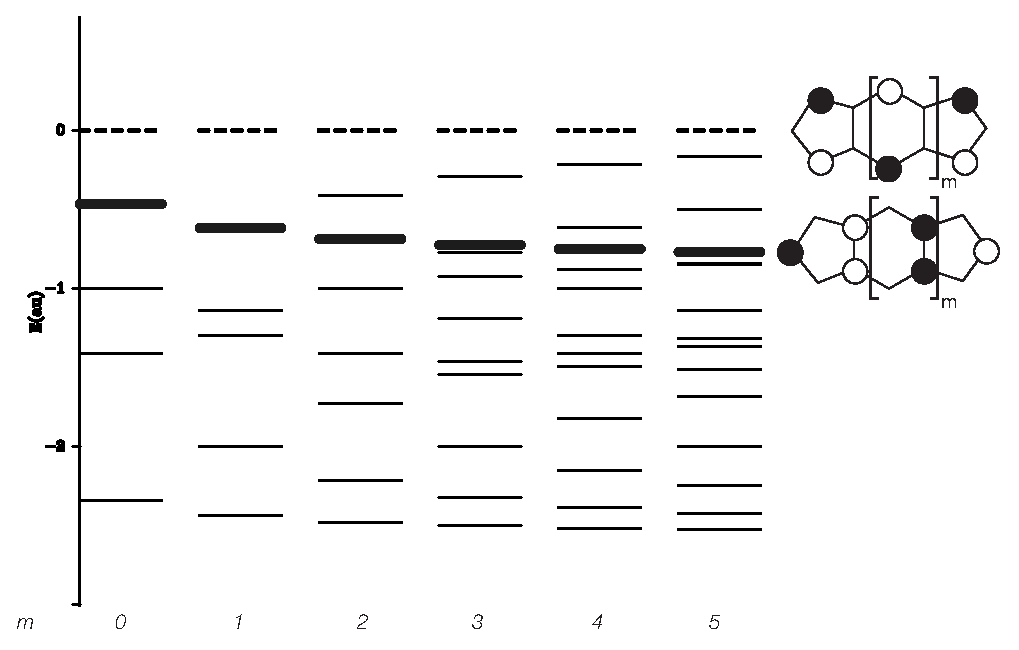
\includegraphics[width=5.5in]{indacene/figures/figure5.eps}
\caption{H\"uckel molecular orbital energies of the bonding MOs for the series \textbf{1}(\textit{n}). Occupied ($b_\mathrm{3u}$/$b_\mathrm{2g}$ for even/odd $n$) and unoccupied LUMO ($a_\mathrm{u}$/$b_\mathrm{1g}$ for even/odd $n$) orbitals formally drive from the HOMO/LUMO pair of the parent monocycle are indicated by the bold, and dashed lines, respectively.}
\label{ch7.fig05}
\end{figure}
A smooth decrease in energy of the occupied orbital is seen upon chain-elongation, as a consequence of the increasing number of cross-link bonding interactions, leading to a growing gap between this orbital and the fixed-energy LUMO, implying a decrease of paratropic contribution to the ring current.

\subsection{Valence Bond Calculations}

Another view at the behavior of these series is offered by the Valence Bond method, which allows a direct assessment of the resonance energy, and the consequences of resonance for the electronic structure. Valence Bond theory provides information on the bonds in terms of spin-couplings, as the wave function is written as a linear combination of Lewis-type structures. Weights ($W$), summing to unity  \cite{r37}, can be attributed to the individual structures, which provide information about their importance in the total VB wave function.

Three different kinds of Valence Bond calculations were performed. In Figure \ref{ch7.fig06}a-d, the different structures included in the various calculations, are explicitly shown for compound \textbf{1}(\textit{1}); a similar partition scheme was used for the other compounds of the series.
\begin{figure}[ht]
\center
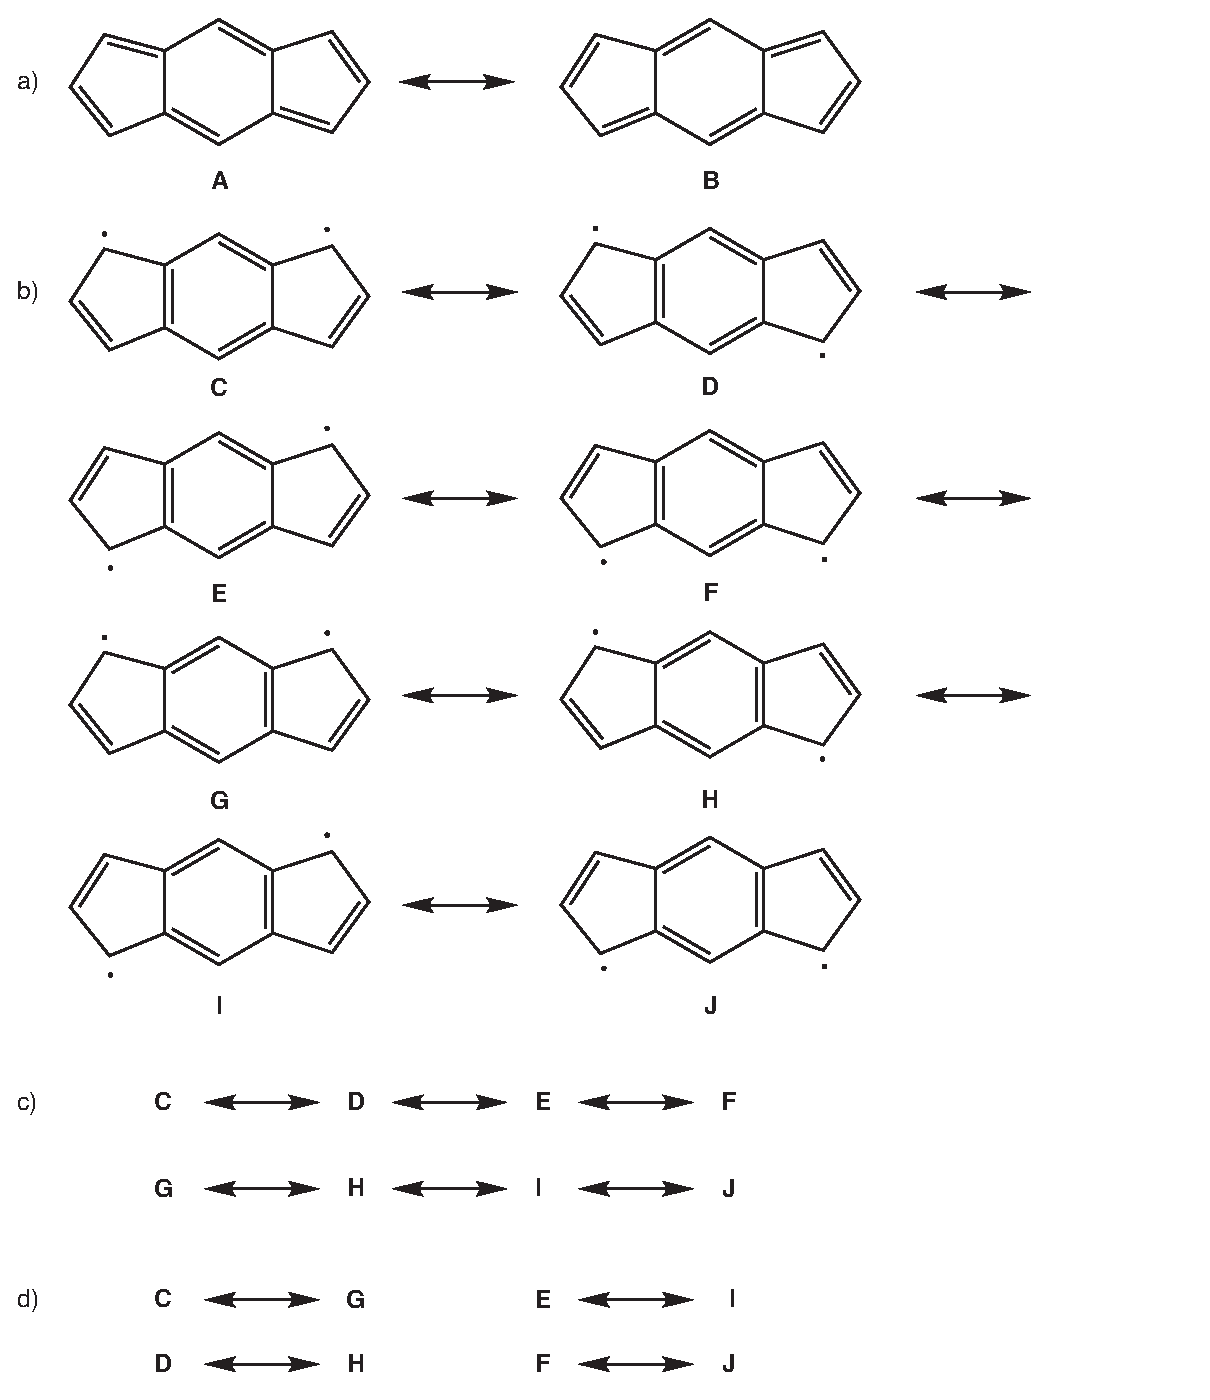
\includegraphics[scale=0.65]{indacene/figures/scheme1.eps}
\caption{Explicit schematic representation of the Valence Bond structures considered in the various calculations for compound \textbf{1}(\textit{1}): (a) the two closed-shell Kekul\'e-type structures, (b) bi-radical allyl-polyacene-like structures, (c) combination of the different allyl structures with an acene structure, to estimate the resonance energy of the allyl moiety, and (d) combination of the different polyacene-structures with identical allyl end groups, to estimate the resonance energy of the polyacene moiety.}
\label{ch7.fig06}
\end{figure}

One calculation was performed where only the two Kekul\'e structures were included (its energy is denoted by $E^\mathrm{VB}_\mathrm{Kek}$, see Figure \ref{ch7.fig06}a), another with all possible bi-radical structures (energy $E^\mathrm{VB}_\mathrm{rad}$, Figure \ref{ch7.fig06}b). To obtain estimates of the resonance energies of the allyl groups and the polyacene moieties, calculations were performed with different Valence Bond structures; either the allyl end groups were allowed to resonate (giving resonance energy $E^\mathrm{allyl}_\mathrm{res}$, Figure \ref{ch7.fig06}c), or only the polyacene moiety was allowed to resonate (giving $E^\mathrm{acene}_\mathrm{res}$, Figure \ref{ch7.fig06}d). Only small energy differences are expected between the estimated resonance energies using the different possible choices of resonating Valence Bond structures of the allyl end groups and the polyacene moiety (Figure \ref{ch7.fig06}c/d). The obtained resonance energies from the symmetry inequivalent sets were averaged. Finally, a calculation that included all the structures depicted in Figure \ref{ch7.fig06}  was performed (energy $E^\mathrm{VB}_\mathrm{tot}$, and resonance energy $E^\mathrm{tot}_\mathrm{res}$).

In Table \ref{ch7.tab03}, a summary of the results of the VB calculation in which all structures were included is given, together with the energies of one of the two Kekul\'e structures ($E^\mathrm{struc}_\mathrm{Kek}$) and of the lowest lying bi-radical structure ($E^\mathrm{struc}_\mathrm{rad}$).
\begin{table}[ht]
\caption{The summed weights ($W$) in the VB wave function of the Kekul\'e structures ($\Sigma W_\mathrm{Kek}$) and bi-radical allyl-polyacene-like structures ($\Sigma W_\mathrm{rad}$), resonance energies $E^\mathrm{tot}_\mathrm{res}$ (in kJ/mol) of molecules \textbf{1}(\textit{n}), and the structure energies (in $E_\mathrm{h}$) of one of the closed-shell Kekul\'e-type structures ($E^\mathrm{struc}_\mathrm{Kek}$) and of the energetically most favorable bi-radical structure ($E^\mathrm{struc}_\mathrm{rad}$), and their energy difference (in kJ/mol). The total number of VB structures considered for each compound is indicated between braces in the first column.}
\begin{center}
\begin{tabular}{l l l c c c c }
\hline
Molecule&
$\Sigma W_\mathrm{Kek}$&
$\Sigma W_\mathrm{rad}$&
$E^\mathrm{tot}_\mathrm{res}$&
$E^\mathrm{struc}_\mathrm{Kek}$&
$E^\mathrm{struc}_\mathrm{rad}$&
$E^\mathrm{struc}_\mathrm{Kek} - E^\mathrm{struc}_\mathrm{rad}$\\
\hline
\textbf{1}(\textit{0}) \{6\}  & 0.959 & 0.041 & -66.00 & -306.088921 & -306.017087 & 188.43\\
\textbf{1}(\textit{1}) \{10\} & 0.420 & 0.580 & -90.25 & -458.603782 & -458.522559 & 213.05\\
\textbf{1}(\textit{2}) \{14\} & 0.326 & 0.674 & -142.20 & -611.101868 & -611.034132 & 177.69\\
\textbf{1}(\textit{3}) \{18\} & 0.227 & 0.773 & -167.62 & -763.600200 & -763.533106 & 175.98\\
\textbf{1}(\textit{4}) \{22\} & 0.134 & 0.866 & -184.09 & -916.098032 & -916.036278 & 161.98\\
\hline
\end{tabular}
\end{center}
\label{ch7.tab03}
\end{table}
The results show that the combined weight of the two Kekul\'e structures decreases with increasing $n$, and conversely the bi-radical character of the compounds increases. The closed-shell Kekul\'e structures remain lower in energy than the radical structures, but by an amount that decays slowly with increasing $n$. The total resonance energy increases with increasing chain-length. Table \ref{ch7.tab04} gives the total energies obtained for the Valence Bond calculations that included all structures, only the Kekul\'e structures and only the bi-radical structures.
\begin{table}[b]
\caption{Total VB energies (in $E_\mathrm{h}$) for the calculations where all structures are included, where only the two Kekul\'e structures are included, and where only the bi-radical structures are included in the calculation.}
\begin{center}
\begin{tabular}{l c c c}
\hline
Molecule&
$E^\mathrm{VB}_\mathrm{tot}$&
$E^\mathrm{VB}_\mathrm{Kek}$&
$E^\mathrm{VB}_\mathrm{rad}$\\
\hline
\textbf{1}(\textit{0}) & -306.114076 & -306.113146 & -306.055910 \\
\textbf{1}(\textit{1}) & -458.638192 & -458.615101 & -458.608609 \\
\textbf{1}(\textit{2}) & -611.156074 & -611.106011 & -611.132970 \\
\textbf{1}(\textit{3}) & -763.664104 & -763.602100 & -763.648898 \\
\textbf{1}(\textit{4}) & -916.168221 & -916.098564 & -916.159471 \\
\hline
\end{tabular}
\end{center}
\label{ch7.tab04}
\end{table}
$E^\mathrm{VB}_\mathrm{Kek}$ is lower than $E^\mathrm{VB}_\mathrm{rad}$ for \textbf{1}(\textit{0}) and \textbf{1}(\textit{1}), but higher for the higher homologues. This indicates that the two smallest molecules in the series are better described by closed-shell structures, but that the others are better described by bi-radical structures. The increasing preference for bi-radical structures can be explained by the growing resonance energy of the polyacene moiety. As seen in Table \ref{ch7.tab05}, the allyl resonance energy ($E^\mathrm{allyl}_\mathrm{res}$) varies hardly at all with increasing $n$, while $E^\mathrm{acene}_\mathrm{res}$ steadily increases.
Thus for the larger members of this series, it becomes energetically favorable to go from the lowest energy, closed-shell, structure to a bi-radical structure, owing to the gain in the $E^\mathrm{acene}_\mathrm{res}$.
\begin{table}[ht]
\caption{Estimates of the resonance energy (in kJ/mol) of the allyl structures and polyacene structures.}
\begin{center}
\begin{tabular}{l c r}
\hline
Molecule &
$E^\mathrm{allyl}_\mathrm{res}$&
$E^\mathrm{acene}_\mathrm{res}$\\
\hline
\textbf{1}(\textit{0}) & -101.82 &  0.00\\
\textbf{1}(\textit{1}) & -117.00 & -109.27\\
\textbf{1}(\textit{2}) & -119.84 & -140.53\\
\textbf{1}(\textit{3}) & -119.67 & -183.59\\
\textbf{1}(\textit{4}) & -119.72 & -202.10\\
\hline
\end{tabular}
\end{center}
\label{ch7.tab05}
\end{table}

\section{Conclusions}

A computational study of the $\alpha$,$\omega$-bicyclopentadiene-polyacene series shows that larger molecules in this series become gradually more aromatic, despite the fact that all have 4$n$ $\pi$ electrons, and each has only the two closed-shell Lewis structures available to the 4$n$ monocycles. The sense of circulation of the induced current density by a magnetic field reverses from paratropic to diatropic with increasing chain length. Within the ipsocentric model, this is explained by a stabilization of the HOMO rotational partner of an unaffected LUMO, resulting in a decrease of the paratropic contribution. Insertion of new energy levels leads to diatropic contributions to ring current of increasing intensity.

The Valence Bond calculations show that the gain in resonance energy by adopting an allyl-polyacene-like structure counteracts the cost of formation of a bi-radical. In line with the ring current criterion for aromaticity, this demonstrates that upon chain lengthening the aromatic character of the $\alpha$,$\omega$-bicyclopentadiene-polyacene series increases.

\section*{Acknowledgements}

Presented at the ESF Exploratory Workshop: New Perspectives on Aromaticity, Exeter, UK, July 5--9, 2003. We gratefully acknowledge partial financial support from NWO/NCF for use of supercomputer time on TERAS, SARA (The Netherlands, project number \mbox{SG-032}).

\bibliography{indacene}
\bibliographystyle{../main/achemso}
